%\documentclass[pdflatex,11pt]{aghdpl}
% \documentclass{aghdpl}               % przy kompilacji programem latex
\documentclass[pdflatex,en]{aghdpl}  % praca w jzyku angielskim
\usepackage[latin2]{inputenc}
%\usepackage[polish]{babel}

% dodatkowe pakiety
\usepackage{enumerate}
\usepackage{listings}
\usepackage{algorithmic}
\usepackage{graphics}
\usepackage{float}
%\usepackage[pdftex]{graphicx}
\usepackage{amsmath}
\usepackage{appendix}
\usepackage[lined,boxed,commentsnumbered]{algorithm2e}
\usepackage{braket}



\lstloadlanguages{TeX}

%---------------------------------------------------------------------------

\author{Krzysztof Doroz}
\shortauthor{K. Doroz}

\titlePL{Zastosowanie wieloagentowych algorytm\'ow koewolucyjnych w problemie optymalizacji portfolio.  }
\titleEN{Application of Co-Evolutionary Multi-Agent Algorithms for Portfolio Optimization Problem}

\shorttitlePL{Zastosowanie wieloagentowych algorytm\'ow koewolucyjnych w problemie optymalizacji portfolio.  } % skrona wersja tytuu jeli jest bardzo dugi
\shorttitleEN{Application of Co-Evolutionary Multi-Agent Algorithms for Portfolio Optimization Problem}

\thesistypePL{Praca magisterska}
\thesistypeEN{Master of Science Thesis}

\supervisorPL{dr in\.z Rafa\l{} Dre\.zewski}
\supervisorEN{Rafa\l{} Dre\.zewski Ph.D}

\date{2011}

\departmentPL{Katedra Informatyki}
\departmentEN{Department of Computer Science}

\facultyPL{Wydzia\l{} Elektrotechniki, Automatyki, Informatyki i Elektroniki}
\facultyEN{Faculty of Electrical Engineering, Automatics, Computer Science and Electronics}

\acknowledgements{Serdecznie dzi\k{e}kuj\k{e} Panu Promotorowi dr. in\.z. Rafa\l{}owi Dre\.zewskiemu za wiele cennych wskaz\'owek podczas pisania pracy magisterskiej}


\setlength{\cftsecnumwidth}{10mm}

%---------------------------------------------------------------------------

\begin{document}

\titlepages

\tableofcontents
\clearpage

\chapter{Introduction}
\label{cha:introduction}

The portfolio optimization problem is of paramount importance to each investor willing to risk their money in order to get potential benefits exceeding interest rates.
Before 1950s, people relied on common sense, experience or even premonition to construct their portfolio.
Then the scientists were able to formulate theories establishing the relation between risk and potential return of the investment.
Finally, investors had solid tools at hand to ease the uneasy process of investing money.
Obviously proposed theories will not make each of us a millionaire.
They can merely be used as a yet another source of analytical information that can be taken into consideration.

My thesis focuses on apllication of co-evolutionary multi-agent algorithms to solve the portfolio optimization problem.
Co-evolutionary algorithms are a large group of methods, which are mimicking natural process of evolution, solving optimization problems.
In order to even closer reflect the natural populations of living creatures, we basically introduce independent entities simulating interactions and behaviour of real creatures
competing for resources in a natural habitat.
That level of flexibility can be obtained by using multi-agent approach.

Finally, some tests have been performed to verify whether the proposed approach would perform well confronted with historical data. 
     


%---------------------------------------------------------------------------

\section{Main goals}
\label{sec:mainGoals}

The main goal of this thesis is to find and apply efficient methods od solving the portfolio optimization problem. That task can be further split into three main steps.

First of all, it was necessary to find some robust methods of solving multi-objective optimization problems that would be appropriate to the problem mentioned in the thesis topic.

Secondly, all approaches selected to be feasible in the first step had to be adjusted to actually solve the portfolio optimization problem.
Most of the selected algorithms give only a vague idea of how to deal with a general optimization problem so it was necessary to actually implement and adapt them to this
 particular problem.

Finally, the tests based on historical data have been performed to assess the performance of each approach.

%---------------------------------------------------------------------------

\section{Content overview}
\label{sec:zawartoscPracy}

Detailed description of multi-objective optimization and portfolio optimization problem are covered in chapter \ref{cha:multiObjectiveOptimization}.
Apart from that, Capital Asset Pricing Model, which is further used as a basis for fitness functions formulation, and all algorithms that have been implemented are described.
That involves: trend following basics, co-evolutionary algorithms with particular emphasis on genetic algorithms.
Finally, the co-evolutionary multi-agent system is described in great detail.

Chapter \ref{cha:implementedAlgorithms} discusses all implementation details of used algorithms.
The description is especially focuses on modifications of general approaches described in chapter \ref{cha:multiObjectiveOptimization} to solve the portfolio optimization problem.

Information regarding technical details of running and modifying implemented algorithms are provided in appendix \ref{cha:user_guide}.

Test results are presented in chapter \ref{cha:tests}. 
Implemented algorithms have been tested on historical data so their performance can be compared with each other.













%\chapter{Basic Definitions}
\label{cha:basic}


%---------------------------------------------------------------------------

\begin{description}
  \item [JMS]
	Java Message Service, it allows application to create, read, send and receive messages.
	Implementations of JMS provide reliable and asynchronous communication for distributed systems. 

  \item [portfolio]
	Portfolio is a collection of investments owned by an investor.
	It could contain many different assets like stocks or bonds.
	Usually the more diversified the portfolio the safer our investments.

  \item [Inversion of Control]
	Inversion of Control (IoC) is an architectural pattern.
	It relies on concept of having an outside entity (usually it is called IoC container) that is responsible for wiring objects together. \cite{Spring} 

  \item [Spring Framework] 
	Spring Framework is a very popular, open source application development framework that makes the process of   application development much easier.
	It contains many useful modules (e.g. IoC container, transaction management, etc.).
	One of its main advantages is lightweight and flexibility. \cite{Spring}

  \item [Java]
	Object oriented programming language that is portable, secure and robust.
	Java code is compiled to byte code interpeted by Java Virtual Machine. 
	It is very popular thanks to ease of application development. 

  \item [population (statistics)]
	Population is a set containing all entities that are relevant in a statistical study of a particular problem \cite{Oxford}. 

  \item [population mean]
	
	The mean of an observation variable is a numerical measure of the central location of the data values.
	The population mean is defined as:
	 \begin{equation}
			\mu = \frac{1}{N} \sum_{i=1}^{N}{(x_{i})} 
		      \end{equation}
  \item [population variance]
	The variance is a numerical measure of how the data values is dispersed around the mean.
	The population variance is defined as:  
	      \begin{equation}
			\sigma^2 = \frac{1}{N} \sum_{i=1}^{N}{(x_{i} - \mu)} 
		      \end{equation}
	where $\mu$ is a population mean.
	   
  \item [population standard deviation]
	The population standard deviation ($\sigma$) is a square root of the population variance.
  \item [covariance]
	The covariance of two variables x and y in a data sample measures how the two are linearly related.
	A positive covariance would indicates a positive linear relationship between the variables, and a negative covariance would indicate the opposite. 
	The population covariance is defined as:

	\begin{equation}
			\sigma_{xy} = \frac{1}{N} \sum_{i=1}^{N}{(x_{i} - \mu_{x})(y_{i} - \mu_{y})} 
		      \end{equation}
	where $\mu_{x}$ and $\mu_{y}$ are population means.

  \item [correlation coefficient]
	Correlation coefficient is a normalized measurement of how the two variables in a data sample are linearly related.
	The population correlation coefficient is defined as:

	\begin{equation}
	  \rho_{xy} = \frac{\sigma_{xy}}{\sigma_{x} \sigma_{y}}
	\end{equation}
	where $\sigma_{x}$ and $\sigma_{x}$ are the population standard deviations and $\sigma_{xy}$ is the population covariance.
	
  
\end{description}


















\chapter{Problem Statement}
\label{cha:multiObjectiveOptimization}



%---------------------------------------------------------------------------

\section{Multi-Objective Optimization}
\label{sec:multi}

The main goal of optimization is to find the very best solution from a most likely infinite set of possibilities.
Optimization procedure relies on finding and comparing feasible solutions until no better solution can be found.
Each solution can be classified as good or bad in terms of a specific objective we are interested in.
E.g. we could define objective as the cost of fabrication, efficiency of a technological process, etc.
Contrary to single-objective optimization there is no clearly defined optimum, instead of that we have to deal with a set of trade-off optimal solutions.
They are generally known as Pareto-optimal solutions (\cite{Phd}).

Vast majority of real-world problems involve more than one objective.
That's why it is so crucial to develop methods to efficiently solve them.
(\cite{Phd}, \cite{Deb:2001:MOU:559152})

\subsection{Formal definition}

Multi-objective optimization problem (MOOP) deals with more than one objective function.
It turns out that objectives are most likely contradictory which makes the MOOP difficult to solve.
In fact it is the most common situation we will ever encounter. 
Following \cite{Deb:2001:MOU:559152} - formal definition of MOOP is being defined as follows:

\begin{equation} 
MOOP \equiv
 \begin{cases}
     Minimize/Maximize  & f_{m}(\bar{x}), \text{ } m = 1,2...,M \\
     Subject \text{ } to  &  g_{j}(\bar{x}) \geq 0, \text{ } j = 1,2..., J  \\ 
			  &  h_{k}(\bar{x}) = 0, k = 0,1...,K \\
			  &  x_{i}^{(L)} \leq x_{i} \leq x_{i}^{(U)}, i = 1,2...,N
      
\end{cases}  
\end{equation}

These constraints and bounds ($g_{j}(x) , h_{k}(x) $ are constraint functions and there are $M$ objective functions) constitute a \emph{decision space}. 
\cite{Deb:2001:MOU:559152}
Any solution that satisfies all the constraints and bounds is called a \emph{feasible solution} \cite{Deb:2001:MOU:559152}.

It turns out that the set of feasible solutions is partially ordered.
In order to compare two solutions we introduce \emph{Pareto dominance} relation \cite{Phd}:

\begin{equation}
\bar{x}_{A}  \prec \bar{x}_{B} \equiv
      \begin{cases}
     \exists{i \in 1..M} : f_{i}(\bar{x}_{A}) < f_{i}(\bar{x}_{B}) \\
     \neg (\exists{j \in 1..M} : f_{j}(\bar{x}_{A}) > f_{j}(\bar{x}_{B}))  \\ 
			  
      
\end{cases} 
\end{equation}

Solution that is not dominated by any other solution is called \emph{non-dominated}. 
The set of \emph{non-dominated} solutions is what we are actually trying to find while dealing with MOOPs.



\begin{figure}[H]
  \begin{center}
    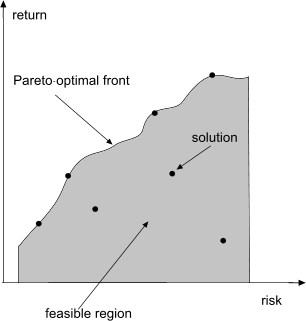
\includegraphics[scale=.9]{pareto_front.png}
  \end{center}
  \caption{Pareto-optimal front of portfolio optimization problem}
\end{figure}


Pareto-optimal front is the set of choices that are \emph{non-dominated} (\cite{Dre}).
 

\subsection{Portfolio Optimization Problem}

Portfolio optimization problem is an example of MOOP.
Portfolio is a set of assets or equities (e.g. stocks) owned by an investor.
Investors cannot rely solely on their intuition to make the right choice.
It is obvious that every investor would like to have the highest return possible.
Unfortunately, equities with high returns usually correlate with high risk. 
That is why it is up to the investor to decide what level of risk are acceptable.

%---------------------------------------------------------------------------

\section{Capital Asset Pricing Model}
\label{CAPM}

%\cite{CAPM}

Modern Portfolio Theory (MPT) (introduced by Harry Markowitz in 1952) was a tremendous breakthrough. 
Investors could finally use a mathemathical approach to construct their portfolios.
Most of them used solely diversification as a mean of reducing portfolio's risk.
With brand new theory they did not have to rely only on common sense - the investment risk was finally expressed in quantitative terms. 

Nevertheless MPT is not perfect, even its creators are fully aware that it has some very important limitations.
The following assumptions of MPT are responsible for its shortcomings [\cite{MPT}]:
\begin{itemize}
  \item variance of portfolio returns is the correct measure of investment risk
  \item investment returns of all assets can be adequately represented by the normal distribution
\end{itemize}

  

Capital Asset Pricing Model (CAPM) was developed in 1960s by Sharpe (\cite{CAPM-Sharpe}) and Lintner.
 
As well as MPT it tries to find the relationship between the price of a single asset and its risk.
Answering the question of how to calculate a risk as well as return of any asset being a part of portfolio is of paramount importance to each investor.

The Sharpe capital asset pricing model is based on the following assumptions \cite{CAPM}:

\begin{itemize}
  \item all investors are risk aversing
  \item all investors have the same information about the market
  \item capital markets are perfect - no transaction costs, no tax, all assets are infinitely divisible
  \item all investors view the expected returns and standard deviations of return provided by different portfolios in the same way
\end{itemize}
 
Lets assume that investor portfolio contains $N$ assets, then according to Capital Asset Pricing expected return of asset $i$ is \cite{CAPM}: 

\begin{equation}
\label{first_eq}
 E(R_{i})  = R_{f} + \frac{ [E(R_{m}) - R_{f}]} {\sigma^2(R_{m})} cov(R_{i}, R_{m})
\end{equation} 

\begin{description}
  \item [$E(R_{i})$]
    expected return of asset $i$
  \item [$R_{f}$]
    risk-free rate of interest (e.g. government bonds)
  \item [$E(R_{m})$]
    expected return of the market
  \item [$\sigma^2(R_{m})$]
    variance of the market return
  \item [$cov(R_{i}, R_{m})$]
    covariance between market return and asset $i$ return
\end{description}

While the risk associated with entire portfolio is equal to:

\begin{equation}
\label{sec_eq}
 \sigma_{p}  = \sqrt{\sum_{i} \sum_{j} w_{i}w_{j} \sigma_{i} \sigma_{j} \rho_{ij}}
\end{equation} 

\begin{description}
  \item [$\sigma_{p}$]
    portfolio risk
  \item [$w_{i}$]
    weighting of component asset $i$
  \item [$w_{j}$]
    weighting of component asset $j$
  \item [$\sigma_{i}$]
    standard deviation of asset $i$
  \item [$\sigma_{j}$]
    standard deviation of asset $j$
  \item [$\rho_{ij}$]
    correlation coefficient between the returns on assets $i$ and $j$
\end{description}
 
%---------------------------------------------------------------------------

\section{Trend following}
\label{sec:trendFollowing}

\subsection{Trend following fundamentals}
\label{sec:trend_following_fundamentals}

The concept of price as the trading cue lays the foundations for trend following (TF). 
Contrary to other trading strategies based on fundamental analysis (which use factors like: overall state of the economy, interest rates, production, etc. to predict stock price)
TF use only price as the key trading variable. 

Trend following basically does not try to predict when the trend will occur. 
Instead of that, trend followers will react to the market's movement and adapt accordingly.
This strategy simply analyses stock prices and decides whether the current situation is suitable for buying or selling a specific stock.
Market breakouts are a great buying opportunities, when you recognize that you are wrong you exit immediately in order to cut losses.
Set of predefined rules decides  whether to take any action (they should recognize when the trend starts as well as when to exit) so the entire process can be easily automated.
Such rules are quite simple but disciplined execution of them could lead to achieving spectacular returns year after year.
It is all about cutting the losses and letting the profits run.
Many leading hedge funds successfully use strategies based on trend following to manage their portfolios. (\cite{Trend01})  

\begin{figure}[H]
  \begin{center}
    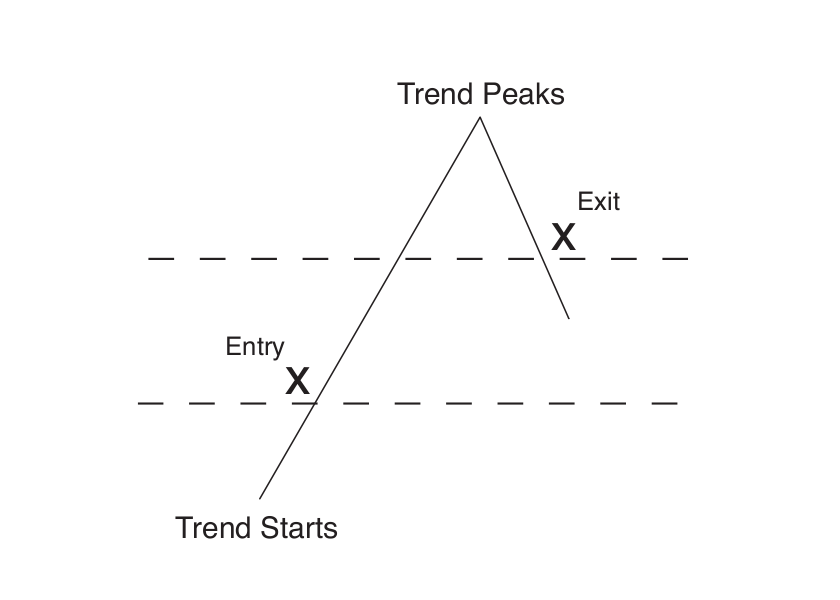
\includegraphics[scale=.4]{trend_following.png}
  \end{center}
  \caption{Simple example of how trend following works in practise}
\end{figure}

Another advantage of this investing method is the fact that investor does not have to know much about what is being traded (it could be stocks, oil, gold, etc.).
Normally, people tend to gather some information about the company they are willing to invest in. 
They analyse its market situation, competitors, financial performance, etc. which is time consuming, especially for someone who is not a professional trader.
With trend following we just have to to focus on elaborating trading rules that should reflect our trading strategy.
After that we can automate the decision making process by designing and implementing our own trading system.   

\subsection{Types of trends}

There are three main types of trends:

\begin{description}
  \item [short-term trend]
      Any price movement that occurs over a few hours or days.
  \item [intermediate-term trend]
      General movement in price data that lasts from three weeks to six months.
  \item [long-term trend]
      Any price movement that occurs over a significant period of time, often over one year or several years.
\end{description}



\subsection{Designing trading system based on trend following} 

Following \cite{Trend01}, the core of each trading system based on trend following strategy is a set of rules governing each buy/sell decision.
More specifically we have to devise rules to answer the following questions:

\begin{itemize}
  \item how much money are we willing to put on a single trade
  \item when to exit (what kind of losses are acceptable)
  \item when to enter (when the trend has started) 
  \item what markets are we interested in and how to split money between them (we would like to have a diverse portfolio (stocks, gold, etc.))
\end{itemize}

These rules should reflect our investing style.

In \ref{trend_following_impl} a system based on trend following strategy is presented in more details.

%---------------------------------------------------------------------------

\section{Evolutionary Algorithms}
\label{sec:evolAlgorithms}

Each stochastic optimization method based on a simulation of evolution process (natural evolution is simulated by an iterative computation process)
can be termed as the Evolutionary Algorithm (EA).
Most commonly known examples of EA include genetic algorithms and evolutionary programming.
A set of candidate solutions, which is modified by the principles of evolution (selection and variation), is used by all above approaches.
Some of solutions present in the population set are better than others (we can assign a fitness value to each solution).
The fitter the solution the more likely it will reproduce.
By means of recombination and mutation new chromosomes are introduced into existing population.
Despite the fact that the principles are quite simple, the resulting algorithm is a powerful search mechanism.  

Apart from all advantages mentioned above, evolutionary algorithms are especially usefull to solve \emph{Multi Objective Optimization Problems} because they
can find multiple \emph{non-dominated} solutions at once. 
According to some researchers evolutionary algorithms are much better suited for MOOPs than strategies based on blind search \cite{Phd}.

\subsection{Basic Principles of Evolutionary Algorithms}

Following \cite{Phd}, EA can be characterized by:

\begin{itemize}
  \item set of possible solutions is kept throughout the algorithm execution
  \item selection process (low quality individuals are removed while well fitted are allowed to reproduce)
  \item set of possible solutions is manipulated by genetic operators (e.g. mutation and recombination)
\end{itemize}

Solution candidates are usually called \emph{individuals} and the entire set of them is called a \emph{population}. 
   
\section{Co-evolutionary Algorithms}
\label{sec:co-evol}

Co-evolutionary algorithms rely on process of co-evolution (two or more species coexist and interact in the same environment).
Individuals of one species interact with each other as well as with members of other species (which simulates the process of adaptation of different species cohabitating the same 
ecosystem).
  
Following \cite{Dre}, co-evolutionary interactions could include:

\begin{itemize}
  \item competition for limited resources
  \item predator-prey interactions
  \item host-parasite interactions
  \item mutualism
  \item commensalism
\end{itemize}

The fitness of each individual simultaneously depends on fitness of the solution as well as other individuals' quality.
The biggest advantage of co-evolutionary algorithms is their ability to maintain population diversity which is crucial to obtain many good solutions in a single algorithm run.    

  

%-------------------------------------------------------------------------------------------------

\section{Genetic Algorithms}
\label{sec:genAlgorithms}

Many computational problems require searching through a huge search space.
Such problems can substantially benefit from an effective use of parallelism.
In that case, many different possibilities are explored simultaneously. 
It turns out that the process of biological evolution could provide an efficient method for addressing these problems.(\cite{Mitchell01})
Because of this genetic algorithms belong to a class of Evolutionary Algorithms (\ref{sec:evolAlgorithms}).


The principles of genetics and natural selection lay the foundations for genetic algorithms (GAs).
GAs are very powerfull tool to solve search and optimization problems.

GAs rely on an evolving population composed of many individuals trying to maximize their \emph{fitness} (i.e., maximizes the return, minimizes cost of fabrication).  
The method was developed by John Holland (1975) over the course of the 1960s and 1970s.(\cite{Haupt:2004:PGA:1007746})

\subsection{Elements of genetic algorithms}

Almost all genetic algorithms have some elements in common \cite{Mitchell01}:
\begin{itemize}
  \item populations of chromosomes
  \item selection according to fitness
  \item crossover to produce new offspring
  \item random mutation of new offspring
  \item fitness function
\end{itemize}

\begin{figure}[H]
  \begin{center}
    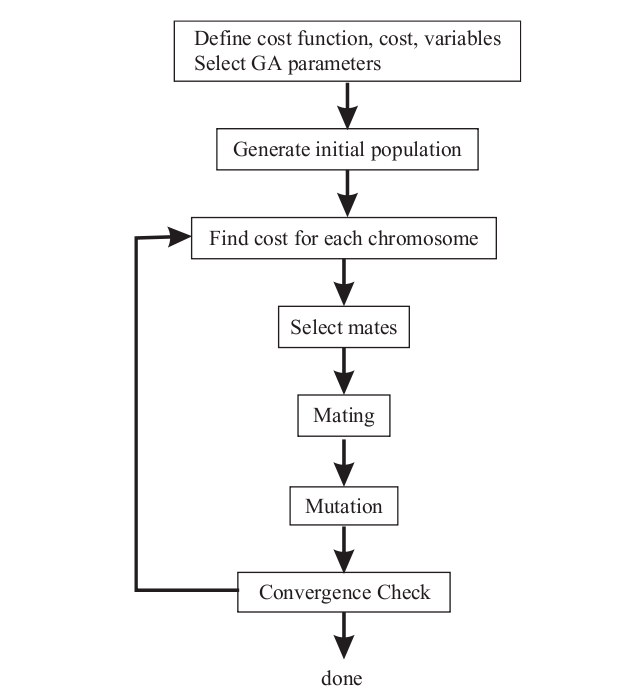
\includegraphics[scale=.4]{GA_flow.png}
  \end{center}
  \caption{GA flow chart \cite{Haupt:2004:PGA:1007746}}
\end{figure}

The GA operates on populations of chromosomes, successively changing one such population to another (by using GA operators: mutation, selection, crossover, etc.). 
Each chromosome contains potential solution to a problem (e.g. represented as binary string). 
Fitness functions are used to assess how well specific chromosome solves the problem.
The better fitting chromosomes are more likely to be involved in reproduction process.
That mimics the biological process of evolution - fitness of an organism is obtained by means of random variation (mutation, recombination, etc.) and natural selection
thus propagating genetic material to future generations.
These rules seems to be simple but they are in fact responsible for extraordinary variety and complexity of the biosphere.
\cite{Mitchell01} 
 
According to \cite{Mitchell01} , high parallelism, discovering and emphasizing solutions that are already quite good are the main reason why GAs work.  
 

\subsection{Genetic algorithms operators}

Following \cite{Mitchell01} - the simplest form of genetic algorithm involves three types of operators: selection, crossover and mutation. 

\begin{description}

\item[selection]
  This operator is responsible for selecting chromosomes from the population for reproduction.
  Likelihood of being chosen is based on the value of fitness function (the fitter the chromosome the better).
  
\item[crossover]
  The crossover operator is responsible for exchanging genetic material between chromosomes.
  Implemantation involves cutting points selection and then cut parts of chromosomes are exchanged.

\item[mutation]
  This operator introduces random changes to a chromosome.
  The probability of random change introduction is usually very small.  

\end{description}

%---------------------------------------------------------------------------

\section{Multiagent Systems}
\label{sec:multi}

There is no universally accepted definition of the term \emph{agent}.
Nevertheless majority of researchers agree that \emph{agent} operates inside some \emph{environment} and should be capable of \emph{autonomous action}.
There is little agreement beyond this. (\cite{Weiss}) 
 
In theory it is possible to imagine a single agent working in an environment but it is quite rare.
The most common situation is a group of autonomous agents interacting inside the environment.
In order to be capable of fulfilling all the above requirements environments have to provide means of communications and interactions to all agents within.

\subsection{Intelligent agents}

The most usefull type of \emph{agents} is called \emph{intelligent agent}.
The \emph{intelligent agent} is capable of (\cite{Weiss}):

\begin{description}
  \item [reactivity]
	  agents can respond to changes in the environment and properly adjust to new conditions
  \item [pro-activeness]
	  agents take the initiative to accomplish their goals
  \item [social ability]
	  agents are capable of intelligent interaction with other agents to satisfy their objectives
\end{description}

\subsection{Co-evolutionary Multi-agent System (CoEMAS)}
\label{sec:CoEMAS}

According to  \cite{Dre} ,\cite{Dre2}, CoEMAS contains the following elements:

\begin{itemize}
  \item the environment 
  \item the set of species that co-evolve 
  \item the set of different resource types (there should be at least one resource type)
\end{itemize}

  
Additionally we define the set of actions that agent can perform :

\begin{description}
  \item [die]
      agent dies when the amount of resources it helds is too low to sustain life (freed resource is given back to environment)
  \item [accept]
      agent accepts partner for reproduction (only agents having more than threshold amount of resources are taken into account)
  \item [give]
      agent is obliged to give some resource to other agent
  \item [get]
      agent is allowed to get some resource from other agent
  \item [seek]
      agent finds another agent so actions like get and finding appropriate partner for reproduction can be perform
  \item [clone]
      action of producing offspring - some amount of resources is passed to newly created agents from parents
  \item [mutation]
      this action is responsible for mutating the agent (introduces random genetic change)
  \item [migration]
      agent is allowed to migrate from the current node to another
  \item [recombination]
      recombination operator is applied
      
\end{description}


\chapter{Implemented Algorithms}
\label{cha:implementedAlgorithms}


%---------------------------------------------------------------------------

\section{Trend following}
\label{trend_following_impl}

The crux of the trend following method is to choose a set of entry and exit point conditions that determine our trading strategy.
Simple Moving Average (SMA) is especially useful to highlight longer-term trends in a set of data points.

SMA is formulated as the unweighted mean of the previous $N$ data points:

\begin{equation}
    SMA_{today,N} = \frac{\sum_{i=1}^{N}p_{today - i}}{N}
\end{equation}

\begin{description}
  \item [$p_{j}$] 
    value of data on day $j$
\end{description}


\textbf{Entry points:}
  \begin{itemize}
    \item Simple moving average (SMA) of last $N$ days is greater than SMA of last $M$ days
    \item Current stock price is max of last $N$ days
  \end{itemize}

As soon as at least one of the above conditions is satisfied we go long.


\textbf{Exit points:}
  \begin{itemize}
    \item Losses on a single trade are greater than 2 \% 
    \item Simple moving average (SMA) of last $N$ days is lesser than SMA of last $M$ days
  \end{itemize}

As soon as the exit condition is satisfied we go short.
 
\subsection{Pseudocode}

\begin{description}

\item[SMA(i,N)]
  calculates Simple Moving Average for stock $i$, $N$ last days are taken into account  
\item[go\_short(i)]
  sell stock $i$
\item[go\_long(i)]
  buy stock $i$
\item[get\_current\_stock\_price(i, day)]
  returns stock $i$ price for specific $day$ 
\item[get\_most\_recent\_trade\_price(i)]
  returns the price we paid for stock $i$ (we have stock $i$ in our portfolio)
\item[max(i,N)]
  returns the maximum price for stock $i$ in the last $N$ days
\item[N, M, maximal\_value\_loss]
  parameters 
\end{description}
% 


\begin{algorithmic}

\STATE $maximal\_value\_loss \gets 0.98$

\FOR{$day = 1$ to $max\_day$} 

  \FOR{$i = 1$ to $number\_of\_stocks$}

    \IF {$ get\_most\_recent\_trade\_price(i) < maximal\_value\_loss * get\_current\_stock\_price(i, day) $} 
	    \STATE $go\_short(i)$
    \ELSE
	    \IF {$SMA(i,N) < SMA(i,M)$}
		    \STATE $go\_short(i)$
	    \ENDIF
    \ENDIF

    \IF {$SMA(i,N) > SMA(i,M)$} 
	    \STATE $go\_long(i)$
    \ELSE
	    \IF {$max(i,N)) < get\_current\_stock\_price(i, day)$}
		    \STATE $go\_long(i)$
	    \ENDIF
    \ENDIF

  \ENDFOR

\ENDFOR

\end{algorithmic}

\subsection{R}

R is a programming language designed to deal with building systems based on statistical computation.
Apart from that it offers command line interpreter.
Working with vectors and matrices of data is straightforward and robust.
Its robustness and vast library of already implemented statistical functions are the main advantages of R (\cite{R}).    

\section{Genetic Algorithm}
\label{sec:genAlgoImpl}

\subsection{Adjusting GA to solve portfolio optimization problem}

As described in \ref{sec:genAlgorithms} each potential solution shoul be encoded in chromosome. 
Each chromosome represents portfolio composition (it is a vector of double values representing percentage share of each stock).

The following modified GA operations have been implemented:
\begin{description}
  \item [mutation]
      Mutation operator changes exactly one value $ \alpha_{i} $ representing percentage share of a specific stock $i$ (each time the value $i$ is chosen randomly)
      to $\alpha_{i}'$ ($\alpha_{i}' \in (0,1)$ is chosen randomly). 
      After that we have to normalize vector.
      $Mutation\_coefficient$ ($mutation\_coefficient \in (0,1)$ ) determines what part of population will be subjected to mutation operator.
  \item [selection]
      $breeding\_coefficient$ ( $breeding\_coefficient \in (0,1)$ ) determines what part of population will be subjected to crossover operator, selection is based on 
      fitness function (only the fittest part of the population will be selected)
  \item [crossover]
      After selection chromosomes eligible for reproduction, each pair of chromosomes are subjected to crossover operator. As a result new chromosomes are created (each pair
      produces two new chromosomes) and added to population. Crossover choose points $left$  and $right$ (both are chosen randomly) which cut parent's chromosomes in the following
      way: 
	  \begin{figure}[H]
	    \begin{center}
	      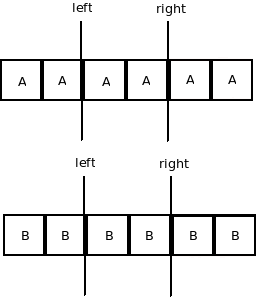
\includegraphics[scale=.4]{parents.png}
	    \end{center}
	    \caption{Example of parent's chromosomes split into 3 parts}
	  \end{figure}

	Now children are created in the following way:    
	  \begin{figure}[H]
	    \begin{center}
	      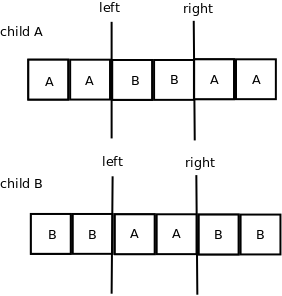
\includegraphics[scale=.4]{children.png}
	    \end{center}
	    \caption{Children's chromosomes contain mixed parent's genetic material}
	  \end{figure}

\end{description}

Apart from that, extinction mechanism has been implemented.
At the end of each GA round a part of the population that has the lowest fitness is exterminated.
$Extinction\_coefficient$ defines what part of population will be subjected to extinction.
 
\subsection{Fitness function}
\label{sec:gen_fitness_fun}

Fitness is calculated according to the following formula (for portfolio with $N$ stocks):

\begin{equation}
    \gamma_{day} =  \sum_{i=0}^{N} {  \alpha_{i} * \frac{price(i,day)}{price(i,day - 1)} }
\end{equation}

\begin{description}
  \item [$\gamma_{day}$] 
      value of the portfolio's fitness calculated for specific $day$
  \item [$\alpha_{i}$]
      percentage share of a specific stock $i$ in the whole portfolio
  \item [$price(i,day)$]
      returns the price of stock $i$ for a specific $day$
\end{description}

Clearly, the fitness function favours the portfolios which have the highest day-to-day increase in value.
Of course such method of calculating fitness has many drawbacks e.g. it completely omits the aspect of risk associated with investing in highly volatile stocks.
However, it turns out that in spite of this obvious flaw the algorithm is performing quite well.  

\subsection{Class Diagram}
\label{gen-class-diagram}

\begin{figure}[H]   
	    \begin{center}
	      \includegraphics[scale=.35]{Simple_gen_UML.png}
	    \end{center}
	    \caption{Class diagram of GA described in \ref{sec:genAlgoImpl}} 
	  \end{figure}

\begin{description}
  \item [GeneticAlgorithmImpl]
    An implementation of IGeneticAlgorithm, it is responsible for calculating the most optimal portfolio
  \item [GeneticAlgorithmUtils]
    Utility class providing methods used by genetic algorithm (like mutating, crossover etc.)
  \item [IDataSource]
    Described in \ref{dataSource}
  \item [Portfolio]
    Class representing potential solution - it stores all the information about our assets and the current value of them.

\end{description}

\section{Co-evolutionary System}
\label{sec:co-evol-sys}

\subsection{Co-evolutionary approach to portfolio optimization problem}

Contrary to \ref{sec:genAlgoImpl}, two subpopulations coexist side by side.
Each individual represent potential solution to portfolio optimization problem.
Risk oriented subpopulation tries to optimize on risk (the lower risk value the better), whereas the return oriented subpopulation tries to maximize expected return.
Usually the greater the expected return the riskier the investment so our solutions will involve some trade-offs.
However that should not startle us, as we have already predicted in \ref{sec:multi} that optimization under such circumstances is not easy.

As presented in figure~\ref{fig:co-evol}, reproduction is allowed only between members of different subpopulations.
Not every member of a particular subpopulation is allowed to reproduce - only the fittest (fitness of a particular member depends on the subpopulation it belongs to - the fittest one
 in one subpopulation would probably be considered as one of the weakest in the other one).
Thanks to this approach the offspring that is created is very diverse. 
Some part of the weakest members of both subpopulations is subjected to extinction.
Because of that we do not end up with too big population full of useless solutions.
In place of extinct members, offspring of the fittest is introduced to both subpopulations.

Apart from that, some members are subjected to mutations in order to maintain subpopulation diversity.
The migration mechanism has the same purpose - to avoid local extrema.
Risk as well as expected return are calculated according to Capital Asset Pricing Model (described in \ref{CAPM}) .


\begin{figure}[H]  
	    \begin{center}
	      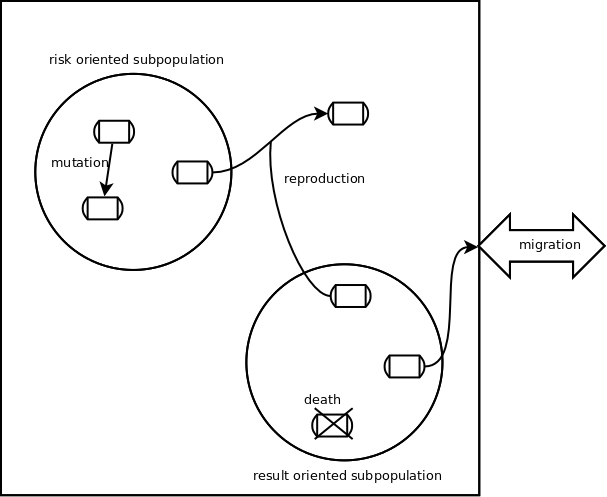
\includegraphics[scale=.35]{co-evol-2-sub.png}
	    \end{center}
	    \caption{Co-evolutionary system overview} 
	    \label{fig:co-evol}
	  \end{figure}

\subsection{Maintaining Population Diversity}

To sum up several mechanisms have been implemented to keep both subpopulations diverse:

\begin{itemize}
  \item crossover is allowed only between the fittest chromosomes from different subpopulations 
  \item mutations introducing random genetic change
  \item migration allows chromosomes to travel to different nodes  
\end{itemize}

\subsection{Class Diagram}
\label{Co-evol-class-diagram}

\begin{figure}[H]   
	    \begin{center}
	      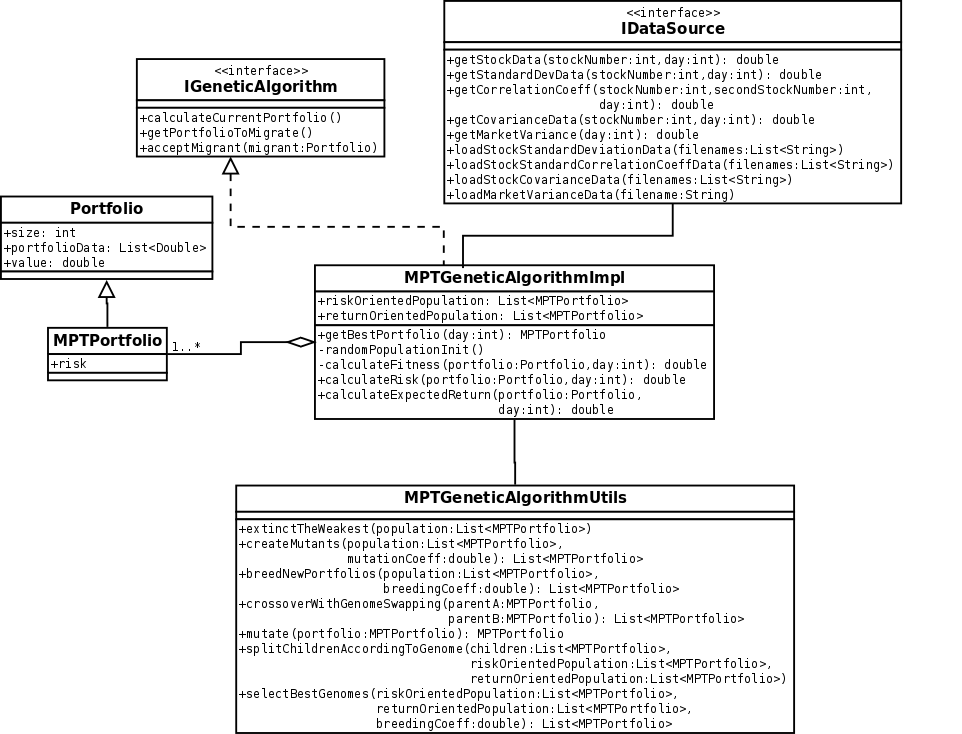
\includegraphics[scale=.35]{co-evol.png}
	    \end{center}
	    \caption{Class diagram of GA described in \ref{sec:genAlgoImpl}} 
	  \end{figure}


\section{Co-Evolutionary Multi-agent System - CoEMAS}

Co-evolutionary Multi-agent System (CoEMAS) is the most sophisticated system that has been implemented.
As described in \ref{sec:multi} and \ref{sec:co-evol} such systems need environment as well as a set of autonomous agents interacting with each other.
Potential solution to portfolio optimization problem is stored inside each agent.


\begin{figure}[H]   
	    \begin{center}
	      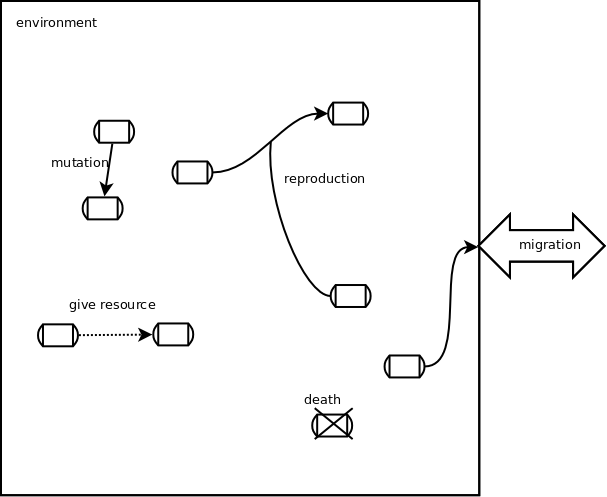
\includegraphics[scale=.38]{agent.png}
	    \end{center}
	    \caption{Overview of CoEMAS} 
	  \end{figure}

Contrary to \ref{sec:co-evol-sys} there are no subpopulations.
Instead of them we introduced individuals of two different species.
Each species focus on different task:

\begin{itemize}
  \item species number 1 - tries to achieve the lowest risk possible
  \item species number 2 - tries to achieve the highest expected return possible
\end{itemize}

Risk as well as expected return is calculated due to Capital Asset Pricing Model (defined in \ref{CAPM}).

Implemented actions that each agent can perform include (\ref{sec:CoEMAS}):

\begin{description}
  \item [death]
      if amount of resource that agent posses is lower than threshold value the agent dies
  \item [migration]
      agent is allowed to migrate but the probability of this action is low
  \item [reproduction]
      agents from different species are allowed to reproduce provided that they both exceed the minimum amount of resource allowing to reproduce
  \item [give/get]
      agent can get resource from other, dominated agent
  \item [recombination]
      agents produce offspring by the means of recombination
  \item [mutation]
      mutation introduces random change to potential solution, normalization of solution vector is then required 
  \item [seek]
      agents appropriate  to reproduction as well as get operation can be found thanks to this action
\end{description}

Interactions between agents are implemented in the following way:
\begin{itemize}
  \item co-evolution is implemented as a sequence of \emph{turns}
  \item in each \emph{turn} every agent perform its action (action to perform at any particular turn is chosen with some well defined probability, e.g. there is a 10\% chance that agent will try to find
	a partner to reproduce, 60\% chance that the agent will try to get some resource from dominated agent)
  \item when every agent performed some action the \emph{turn} ends and entire population of agents is checked whether some of them should die (not enough resource left after other agents got resource
	from it)
\end{itemize}


Each agent performs one of the above actions with some probability.



\subsection{Class Diagram}
\label{CoEMAS-class-diagram}

\begin{figure}[H]   
	    \begin{center}
	      \includegraphics[scale=.3]{CoEMAS-UML.png}
	    \end{center}
	    \caption{Class diagram of CoEMAS} 
	  \end{figure}

\begin{description}
  \item [Environment]
      aggregates all agents, responsible for population init at the start of algorithm and extinction of agents which resource level are too low, etc.
  \item [AgentUtils]
      utility class providing functions to Agent class
  \item [IAgent]
      interface specifying all methods that agent in CoEMAS should be capable of doing
  \item [Agent]
      implementation of agent that is autonomous and interact with other agents
  \item [IDataSource]
      provides easy access to historical data and computed statistical functions
 
\end{description}


%---------------------------------------------------------------------------

\section{Implementation Details}
\label{sec:implDetails}


\subsection{Multi-agent running platform architecture}
\label{multi-agent}

%\clearpage
\begin{figure}[H]
  \begin{center}
    \includegraphics[scale=.4]{agent_framework.png}
  \end{center}
  \caption{Deployment diagram of two Computing Nodes and Aggregation Node (in real situations more Computing Nodes are present)}
\end{figure}

Data Source as well as Computing Algorithm are created and injected to Computing Node(CN) by Spring. 
CNs send results of computations to Aggregating Node by JMS. 
Apart from that, JMS is used to provide migration capability to each CN.


\subsection{Precomputation of statistical functions}
\label{precompute}
Precomputation of statistical functions (like covariance, standard deviation etc.) from historical data is done by R scripts. 
Results are stored in files, later used as an input to other algorithms.
In order to provide easy and centralised access to historical data and precomputed statistical functions Data Source component has been introduced. 

\subsection{Data Source component}
\label{dataSource}

Data Source component aggregates all stocks historical data as well as all precomputed statistical functions results from \ref{precompute}.   
Its interface enables access to all data it contains. Data Source is injected as a bean to other components by Spring.
They use it mainly as a source of data required by various algorithms.

\subsection{Computing Algorithm component}

Computing Algorithm component is responsible for carrying out all computations.
In order to function properly Data Source component as well as all configuration variables (like mutation coefficient etc.) has to be injected by Spring.
Apart from trend following algorithm, all the remaining approaches (CoEMAS (\ref{CoEMAS-class-diagram}), co-evolutionary (\ref{Co-evol-class-diagram}),
 genetic algorithm (\ref{gen-class-diagram})) can be injected to Computing Algorithm component so they can be run
 in a multi-agent system as a working horse of a Computing Node.


\subsection{Aggregating Node}

The sole purpose of Aggregating Node(AG) is to gather results from Computing Nodes(CN), choose the best non-dominated solution and write the results to file. 
Based on this file all charts are created and comparison of different algorithms is possible.
Communication between CNs and AG is provided by a single JMS queue (all CNs send results to one specific queue, AG consumes its content).


\subsection{Technologies used}

\begin{description}
  \item [R]
      Trend following algorithm has been implemented as an R script, historical data preprocessing.
  \item [Apache ActiveMQ]
      JMS implementation, provides communication between Computing Nodes and Aggregating Agent (\ref{multi-agent})
  \item [Java]
      Almost all algorithms are implemented in Java, Computing Nodes as well as Aggregating Node are in fact jar files 
  \item [Spring Framework]
      Inversion of Control container (configuration of application components and lifecycle management of Java objects), Messaging (simplifies the use of the JMS API) modules used.
  \item [Apache Maven]
      Used primarly for build automation.
  \item [JUnit]
      JUnit tests cover the most crucial functions of implemented algorithms.
  \item [git]
      Source Code Management tool.
  \item [bash scripts]
      Used for conveniently setting up and running test 
\end{description}

 
\chapter{Test Results}
\label{cha:pierwszyDokument}

\section{First Set of Tests}
\label{sec:first_set_of_tests}

First set of tests uses historical data from year 2009 (data of 3 different stocks have been used). 
Portfolio contained 3 assets (they are one of the biggest companies present on WSE):

\begin{itemize} 
  \item KGHM
  \item TPSA
  \item PKO
\end{itemize}

Multi-agent platform has been used to run algorithms.
It was configured in the following way: 

\begin{itemize}
  \item configured to simulate trading strategy throughout the entire year 2009
  \item all investing decisions are solely based on results from algorithms
  \item migration mechanism between Computing Nodes has been enabled
  \item two Computing Nodes (with appropriate algorithms) have been used to obtain results
\end{itemize}

Trend following algorithm has been tested without multi-agent running platform as it is a standalone R script.

\subsection{Trend Following}

\subsubsection{Short-term trend results}

As described in \ref{trend_following_impl} and \ref{sec:trendFollowing}, we can adjust our trading rules to seek out short-term trends
 (by changing the values of $N$ and $M$ in the \emph{Simple Moving Average} method).
With values $N = 10$, $M = 20$ the SMA method focused on short-term trends.
 

\begin{figure}[ht]
  
  \begin{center}
    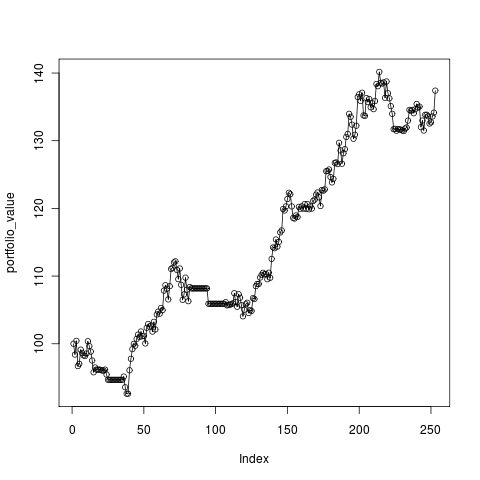
\includegraphics[scale=.4]{rplot0.png}
  \end{center}
  \caption{Chart showing value of our portfolio in time}
  \label{fig:trend-short}
\end{figure}

There are easily visible periods of time (figure~\ref{fig:trend-short}) when the portfolio value is not changing. 
It is a time when our portfolio does not contain any assets (but we still have money). 
After a while, conditions change and trend following algorithm decides to buy some assets.


\subsubsection{Intermediate-term trend results}

In this particular test (with values: $N = 20$, $M = 40$), trend following algorithm has been adjusted to focus on intermediate-term trends.
 
\begin{figure}[H]
  \begin{center}
    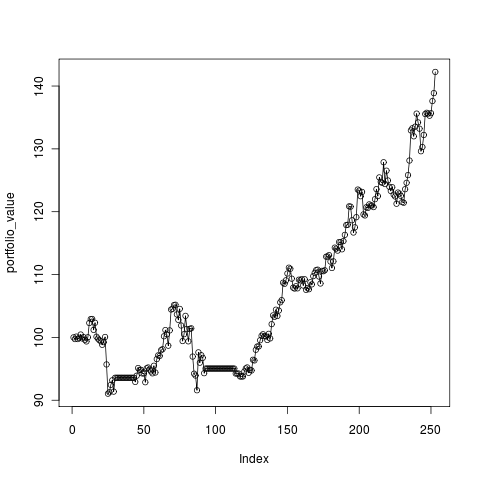
\includegraphics[scale=.4]{rplot.png}
  \end{center}
  \caption{Chart showing value of our portfolio in time}
  \label{fig:trend-int}
\end{figure}

Results are presented in figure~\ref{fig:trend-int}, as can be seen they are slightly better compared with short-term trends approach.  

\subsubsection{Conclusions}

It turned out that focusing on short-term or intermediate-term trends leads to almost the same results.
Intermediate-term trend approach offers slightly better return from the investment.
In both cases we encountered periods of time when portfolio contained no assets because situation on the market was not good enough to invest in any of the available stocks.


%---------------------------------------------------------------------------

\subsection{Genetic Algorithm}

Results are presented in figure ~\ref{fig:gen-algo}.

\begin{figure}[ht]
  \begin{center}
    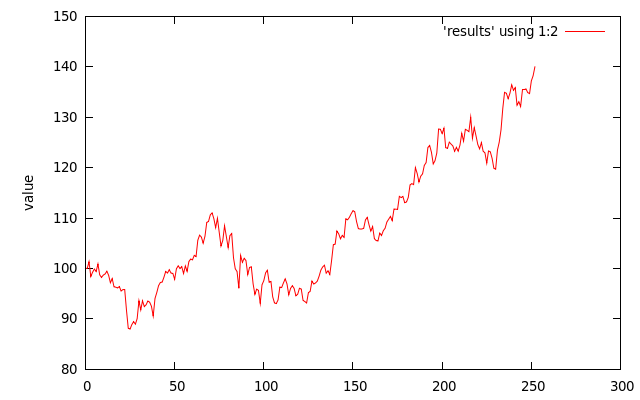
\includegraphics[scale=.5]{simple-genetic-algo.png}
  \end{center}
  \caption{Chart showing value of our portfolio in time}
  \label{fig:gen-algo}
\end{figure}

\subsection{Co-evolutionary algorithm}
\label{sec:co-evol-2}

Results presented in figure~\ref{fig:co_eval_return} clearly show that the return of our investment is much higher than any other algorithm could achieve.  
Analysing figure~\ref{fig:co_eval_risk} explains why the results are so good - the risk associated with our portfolio is substantially higher compared to other methods.
In this case algorithm was tuned to treat non-dominated solutions from return oriented subpopulation - this explains why the results provide so much return and risk. 

\begin{figure}[ht]
  \begin{center}
    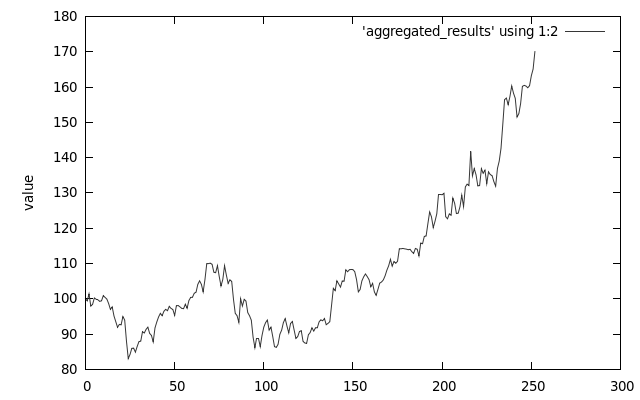
\includegraphics[scale=.5]{co-evol-value-oriented.png}
  \end{center}
  \caption{Chart showing value of our portfolio in time}
  \label{fig:co_eval_return}
\end{figure}

\subsubsection{Pareto front}

Because co-evolutionary algorithm operates in terms of risk and return we can check if the non dominated solutions (in Pareto sense) are used to construct our portfolio.
Figure~\ref{fig:pareto_co_evol} shows the results of computation (results from a period of 6 days are presented for the sake of clarity). 
Portfolio is built according to the solutions that are connected with red line.
All of them are non dominated and all have the maximum return possible from all available feasible solutions at any particular day.

Solutions from two different computing nodes are shown.
It turns out that results from the second node are much better than from the first.
In fact all of the selected solutions come from the second one.

\begin{figure}[ht]
  \begin{center}
    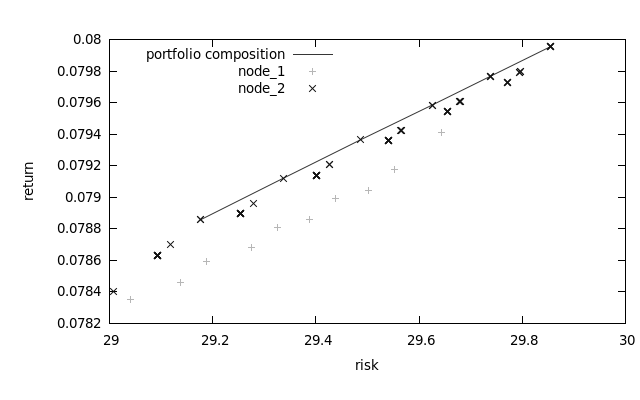
\includegraphics[scale=.5]{pareto_co_evol.png}
  \end{center}
  \caption{Chart showing the relation between return and risk of the particular solution}
  \label{fig:pareto_co_evol}
\end{figure}


\begin{figure}[ht]
  \begin{center}
    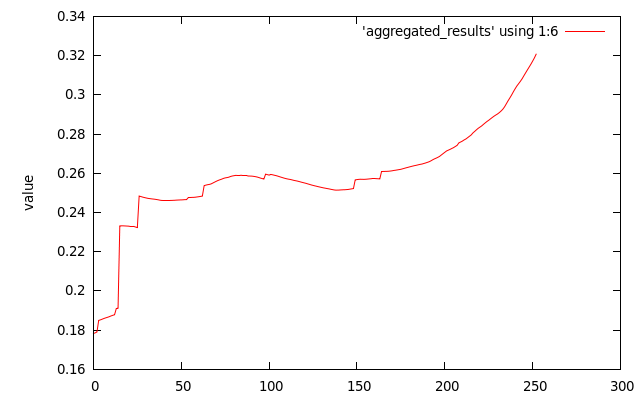
\includegraphics[scale=.5]{co-evol-risk-value-oriented.png}
  \end{center}
  \caption{Chart showing value of risk in time}
  \label{fig:co_eval_risk}
\end{figure}

\subsection{CoEMAS}

Figure~\ref{fig:agent_return} presents portfolio value in time while  figure~\ref{fig:agent_risk} presents the risk associated with our investments.

\begin{figure}[ht]
  \begin{center}
    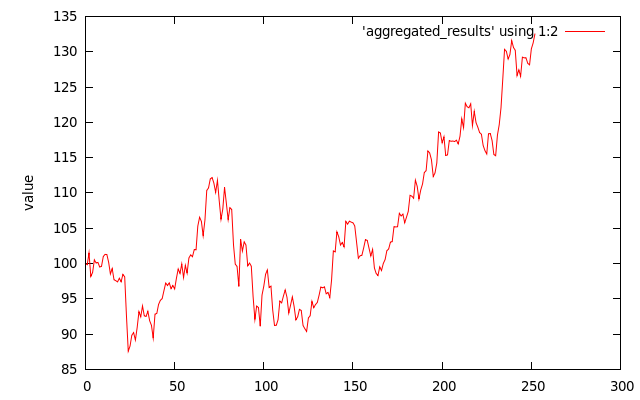
\includegraphics[scale=.5]{agent-return.png}
  \end{center}
  \caption{Chart showing value of our portfolio in time (CoEMAS)}
  \label{fig:agent_return}
\end{figure}

\subsubsection{Pareto front}

CoEMAS like co-evolutionary algorithm gives us the opportunity to check if the non dominated solutions (in Pareto sense) are used to construct our portfolio.
Figure~\ref{fig:pareto_coemas} shows the results of computation (because of the fact that populations are quite numerous,
 results from a period of 3 days are presented for the sake of clarity). 
Solutions chosen to be a blueprint for our portfolio are shown as big black dots.
We can easily spot that they are non dominated (in Pareto sense). 


\begin{figure}[ht]
  \begin{center}
    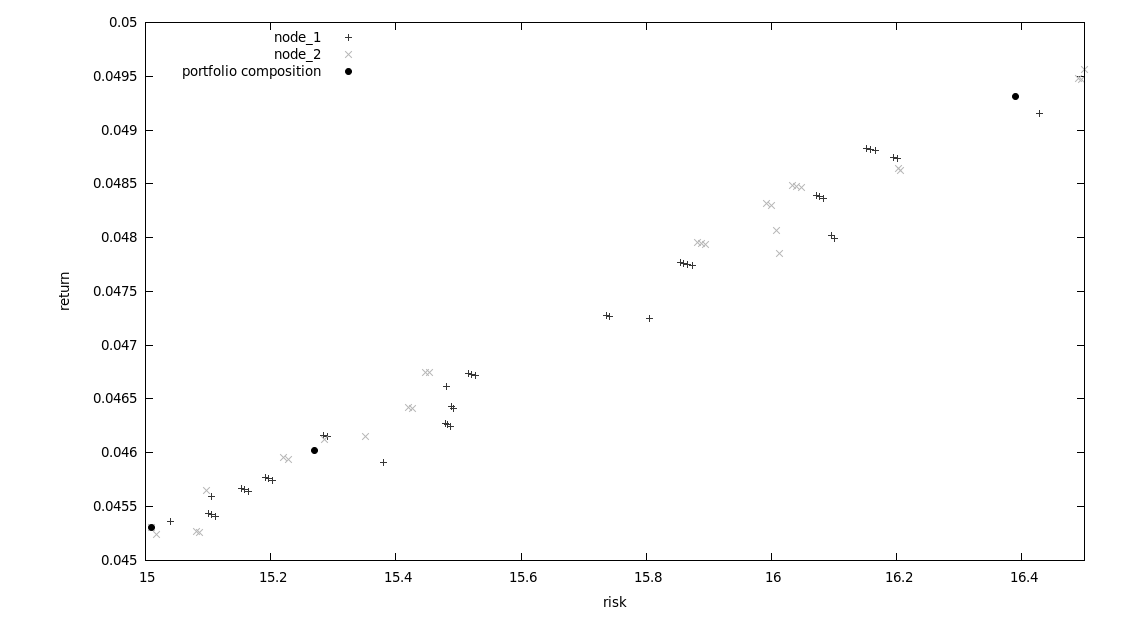
\includegraphics[scale=.4]{pareto_coemas.png}
  \end{center}
  \caption{Chart showing the relation between return and risk of the particular solution}
  \label{fig:pareto_coemas}
\end{figure}

\begin{figure}[ht]
  \begin{center}
    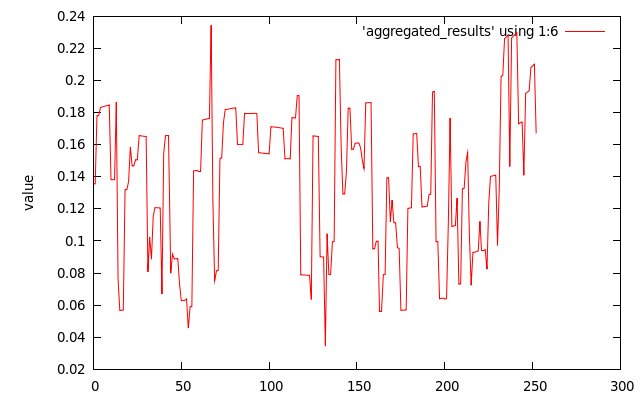
\includegraphics[scale=.5]{agent-risk.png}
  \end{center}
  \caption{Chart showing value of risk in time (CoEMAS)}
  \label{fig:agent_risk}
\end{figure}

\subsection{Conclusions}

First set of tests showed that all algorithms give reasonable results.
It is very hard to pinpoint one approach that is much better than others.
Co-evolutionary system (\ref{sec:co-evol-sys}) outperformed other algorithms in terms of return.
Such good results can be explained by the fact that trading strategy proposed by this algorithm is much riskier than using CoEMAS.
  
On the other hand, CoEMAS offers substantially lower return but is much more safer.
As figure~\ref{fig:agent_risk} shows, the risky moves are mixed with safe ones resulting in much more balanced strategy.

Trend following as well as genetic algorithm can not give us any information about the risk we are taking by investing according to results they provide.
On the other hand, we can specify rules (in the trend following approach) that should reflect our attitude to risk taking (\ref{sec:trend_following_fundamentals}).
With genetic algorithm (GA) we have no such option - as described in \ref{sec:gen_fitness_fun}, our ability to customize GA is limited.
Obviously we could test different values of coefficients responsible for simulating evolution process but it turns out that the fitness function that does not take risk into
account is the most serious limitation.


\section{Second Set of Tests}

The main goal of this set of tests is to chech the impact of increasing the number of computing nodes to the quality of solutions we obtain from implemented algorithms.

Besides the number of computing nodes (now 8 computing nodes will be running at once), the same historical data and configuration has been
 used (as in \ref{sec:first_set_of_tests}) to produce results.



\subsection{Co-evolutionary algorithm}

Figure~\ref{fig:co_evol_8_risk} presents risk associated with our portfolio.


Comparing with results presented in \ref{sec:co-evol-2} we can easily spot that additional computing nodes allowed us to find a solution that is much more risk free.
Apart from that higher number of nodes offer similar performance in terms of return (figure~\ref{co_evol_8_return}).

\begin{figure}[ht]
  \begin{center}
    \includegraphics[scale=.5]{co-evol-8.png}
  \end{center}
  \caption{Chart showing value of risk in time}
  \label{fig:co_evol_8_risk}
\end{figure}

\begin{figure}[ht]
  \begin{center}
    \includegraphics[scale=.5]{co_evol_8_return.png}
  \end{center}
  \caption{Chart showing portfolio value in time}
  \label{fig:co_evol_8_return}
\end{figure}

\subsection{CoEMAS}

\begin{figure}[ht]
  \begin{center}
    \includegraphics[scale=.5]{agent_8_risk.png}
  \end{center}
  \caption{Chart showing portfolio value in time}
  \label{fig:agent_8_risk}
\end{figure}

In case of CoEMAS adding more computing nodes seems to have little effect.
Risk associated with our portfolio is almost the same as before (figure~\ref{fig:agent_8_risk}).
There is no significant improvement in terms of return (as shown in figure~\ref{fig:agent_8_return}). 


\begin{figure}[ht]
  \begin{center}
    \includegraphics[scale=.5]{agent_return_8.png}
  \end{center}
  \caption{Chart showing portfolio value in time}
  \label{fig:agent_8_return}
\end{figure}

\subsection{Conclusions}

Adding additional computing nodes tends to improve the performance of co-evolutionary algorithm, whereas there is almost no impact on CoEMAS.
It can be explained by the fact that each CoEMAS node has a significantly large and diverse population that is not prone to fall in local minima.
Co-evolutionary algorithm benefits a lot from a larger number of computing nodes.  

\section{Third Set of Tests}

\subsection{Trend Following}

\subsubsection{Short-term trend results}
\subsubsection{Intermediate-term trend results}
\subsubsection{Conclusions}

\subsection{Genetic Algorithm}

\subsection{Co-evolutionary algorithm}

\subsection{CoEMAS}


\subsection{Conclusions}
\chapter{Summary}

\section{Main goals}

One of the main goal of this thesis was to find efficient ways of tackling the portfolio optimization problem.
Apart from co-evolutionary multi-agent system, many other approaches have been taken into consideration.
The essential part of work at the beginning consisted of gathering information about any feasible algorithm that could be adjusted to solve the problem. 
The main source of knowledge were books and papers devoted to the identical or very similar problem. 

The second goal was to implement the most promising algorithms found during first stage.
Four genuine approaches have been implemented: genetic algorithm, trend following, co-evolutionary and co-evolutionary multi-agent system.
The last two of mentioned algorithms were run on multi-agent platform. 

Last but not least, all implemented algorithms were supposed to be tested. 
Three sets of tests have been performed in order to assess the usefulness of each of them.


\section{Results}

As mentioned before, four algorithms have been implemented.
Trend following has been implemented as R script.
In case of the other three, Java was used.
Some are run on a multi-agent running platform implemented in Java.
Its architecture seems to be very simple but it provides all functionality that is needed.
Apart from that, to provide user friendliness, a group of shell scripts was created.
They build all necessary artifacts and deploy them.
They are further discussed in appendix A.
   
Three sets of tests have been performed to assess each algorithm performance during substantially different overall situation on a market.
Obtained results showed that it is difficult to pinpoint one approach that outperforms all others.
It is pretty clear that each of them has some pros and cons.
Results are discusses in more detail in chapter \ref{cha:tests}.


\section{Conclusions}

All implemented algorithms have been exhaustively tested using historical data reflecting completely different situations on the market.
Taking into consideration both good and bad times leads to conclusions that all approaches have advantages as well as disadvantages.
That raises a question what algorithm to use if we want to build our own portfolio.
Trend following is good for unstable times because it somehow guarantees that the losses would be minimalised according to our preferences.
However, during stock market rise it is outperformed by other algorithms.
Clearly we would like to have means to highlight good aspects of each algorithm.  
Right now it is a little bit inconvenient therefore new system is proposed in \ref{sec:future}.
That system should expose all strengths of implemented approaches and be user friendly for a casual investor. 


\section{Future work}
\label{sec:future}

All tests have been performed in a way that mimicks real trading on a stock exchange.
Historical stock data have been used, but it is fairly obvious that the systems could be changed to actually invest money in a real world.
Right now the biggest obstacles to efficiently use them are:

\begin{itemize}
  \item feeding data to algorithms is a little bit cumbersome;
  \item each algorithm is implemented as an independent entity;
  \item systems are not user-friendly - running them requires using shell scripts;
  \item modification of algorithms' parameters is inconvenient;
  \item interpreting results is time consuming and could be enhanced.
\end{itemize}
 
New system should combat all the problems mentioned above.
It should incorporate all implemented algorithms and use them as strategies.
Obviously investors should be able to modify parameters of running strategies via user-friendly GUI.
They could set them manually or they could choose from a set of predefined sets of parameters.
User should check what each of them is suggesting and make a decision about a portfolio composition.
Apart from that, access to charts comparing all proposed strategies would be provided.
That should give further insight into situation on the stock market and ease decision making.

All stock data should be downloaded during the start of application from Yahoo! (via YQL - Yahoo Query Language).
After downloading it would be stored in an underlying database.
In that case algorithms could fetch all the data they need (historical as well as most recent one) from one, central database.
 

\chapter{User Guide}
\label{cha:user_guide}



\section{List of scripts}

\begin{description}
  \item [create\_jars.sh]
      It is a script responsible for building jar files of all projects needed to run co-evolutionary algorithm on multi-agent running platform. 
  \item [deploy.sh]
      Script responsible for running co-evolutionary algorithm on a multi-agent platform.
      A special directory called \emph{sandbox} is created and all necessary jar files as well as files containing preprocessed historical data are copied to \emph{sandbox}.
      It also specifies the number of Computing Nodes that will be used for computation.
      ActiveMQ should be started before running this script.
  \item [create\_agent\_jars.sh]
      Script responsible for building jar files of all projects needed to run CoEMAS system on multi-agent running platform. 
  \item [agent\_node\_deploy.sh]
      Script responsible for running CoEMAS system on a multi-agent platform.
      A special directory called \emph{sandbox} is created and all necessary jar files as well as files containing preprocessed historical data are copied to \emph{sandbox}.
      It also specifies the number of Computing Nodes that will be used for computation.
      ActiveMQ should be started before running this script. 
  \item [precompute.R]
      Script responsible for precomputing standard deviation and correlation coefficients from historical data.
  \item [PrecomputeCovVarForMPT.R]
      Script responsible for precomputing covariance and variance from historical data. 

\end{description}



\section{Adjusting Algorithms}

\begin{description}
 \item [trend following]
      In order to adjust trend following algorithm we have to modify the script code.
      Thanks to comments present in code, it is not that difficult.
  \item [genetic algorrithm]
      There are constants (regulating algorithm behaviour) in file GeneticAlgorithmImpl.java that can be set by class constructor. 
  \item [co-evolutionary algorithm]
      Because Spring manages the bean creation of co-evolutionary algorithm, all coefficients responsible for adjusting algorithm behaviour can be set by constructor injection. 
  \item [CoEMAS] 
      CoEMAS can be adjusted in the same way as the co-evolutionary algorithm (constructor injection).
\end{description}


\section{Interpreting results}

Running trend following script will produce results at once - graph, showing portfolio value in time, is plotted as soon as computation is finished.
CoEMAS as well as co-evolutionary algorithm are run in a sandbox and results of the computation are stored in a file.
It contains the information about portfolio composition, total value and risk of portfolio, etc. 
Results from genetic algorithm are stored in a similar way. 





% itd.
% \appendix
% \include{dodatekA}
% \include{dodatekB}
% itd.

\bibliographystyle{amsplain}
\bibliography{bibliography}

\end{document}